\section{Exercise three}

Consider the stochastic process defined by the following diagram:
\begin{figure}[H]
    \centering
    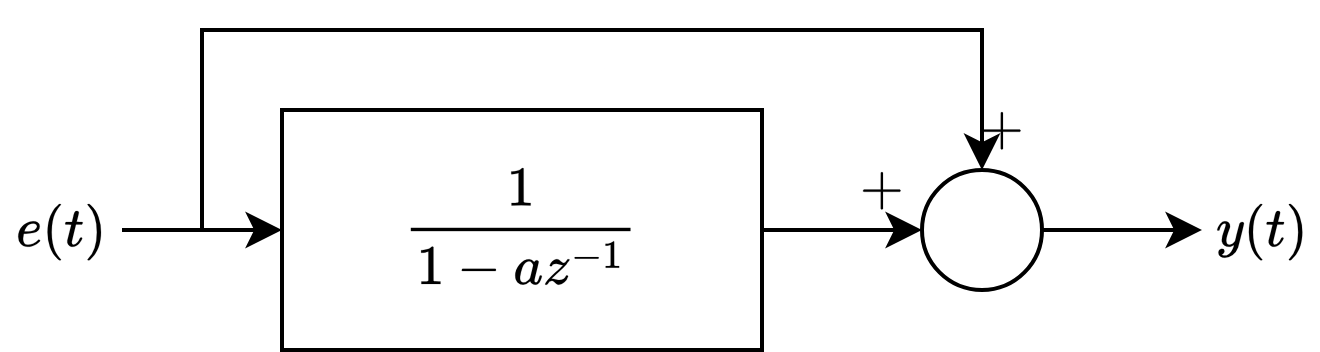
\includegraphics[width=0.5\linewidth]{images/block2.png}
\end{figure}
Here, $e(t) \sim WN(0,\lambda^2)$, and $\left\lvert a\right\rvert <1$.

Find the characteristic values of the given process $y(t)$.

\subsection*{Solution}
To begin, let's compute the expected value of $y(t)$:
\[m_y=\mathbb{E}\left[ y(t) \right]=\mathbb{E}\left[ ay(t-1)+2e(t) \right]=a\mathbb{E}\left[ y(t-1) \right]\rightarrow m_y=0\]

The covariance function at $\tau=0$ is given by:
\[\gamma_y(0)=\mathbb{E}\left[ y(t)^2 \right]=\mathbb{E}\left[ \left(y_1(t)+y_2(t)\right)^2 \right]=\dfrac{4-3a^2}{1-a^2}\lambda^2\]
The covariance function at $\tau=1$ is given by:
\[\gamma_y(1)=\mathbb{E}\left[ y(t)y(t-1) \right]=\dfrac{a\lambda^2(2-a^2)}{1-a^2}\]

Alternatively, noting that we have two processes in parallel with a transfer function equal to:
\[y(t)=\dfrac{1}{1-az^{-1}}e(t)+e(t)=\dfrac{2-az^{-1}}{1-az^{-1}}e(t)\]
The canonical form becomes:
\[y(t)=\dfrac{1-\frac{a}{2}z^{-1}}{1-az^{-1}}e_1(t)\]
Here, $e_1(t)=2e(t)$, implying that $e(t) \sim WN(0,2^2\lambda^2)$.
We can now find the time-domain representation, which is:
\[y(t)=ay(t-1)+\eta_1(t)-\dfrac{a}{2}\eta_1(t-1)\]
From this, we can compute the covariance in a more straightforward manner.